\documentclass{article}
\usepackage{hyperref}
\usepackage{parskip}
\usepackage{caption}
\usepackage{graphicx}

\usepackage{hyperref}
\hypersetup{hidelinks}

\def\version{2.1}

\begin{document}

\title{User Guide for Auto-WEKA version \version}

\author{
Lars Kotthoff, Chris Thornton, Frank Hutter\\
\texttt{\{larsko,cwthornt,hutter\}@cs.ubc.ca}
}

\maketitle

\tableofcontents

%%%%%%%%%%%%%%%%%%%%%%%%%%%%%%%%%%%%%%%%%%%
\section{Introduction}\label{sec:intro}
%%%%%%%%%%%%%%%%%%%%%%%%%%%%%%%%%%%%%%%%%%%

Auto-WEKA is a tool that performs combined algorithm selection and hyperparmeter
optimisation over the classification and regression algorithms implements in
WEKA. More specifically, given a specific dataset, Auto-WEKA explores
hyperparameter settings for many algorithms and recommends to a user which
method will likely have good generalization performance, using model based
optimisation techniques.

\subsection{Availability}

Auto-WEKA is available as a WEKA package through the WEKA package manager (WEKA
version 3.7.13 and later). The source code is available at
\url{https://github.com/larskotthoff/autoweka}, where bugs can be reported as
well.

%%%%%%%%%%%%%%%%%%%%%%%%%%%%%%%%%%%%%%%%%%%%%%%%%%%%%%%%%%%%%%%%%%%%
\subsection{License}
%%%%%%%%%%%%%%%%%%%%%%%%%%%%%%%%%%%%%%%%%%%%%%%%%%%%%%%%%%%%%%%%%%%%

Auto-WEKA is open source software issued under the
\href{http://www.gnu.org/licenses/gpl.html}{GNU General Public License}. Note
that the included SMAC optimisation method is licensed under the AGPLv3.

\subsection{Requirements}

Auto-WEKA does not have any additional requirements compared to WEKA. If you can
run WEKA, you should be able to run Auto-WEKA.

%%%%%%%%%%%%%%%%%%%%%%%%%%%%%%%%%%%%%%%%%%%
\section{Auto-WEKA Overview}\label{sec:overview}
%%%%%%%%%%%%%%%%%%%%%%%%%%%%%%%%%%%%%%%%%%%

Auto-WEKA is used much like any other WEKA classifier. After loading a dataset
into WEKA, it can be run on it to automatically determine the best WEKA model
and its parameters.

%%%%%%%%%%%%%%%%%%%%%%%%%%%%%%%%%%%%%%%%%%% 
\subsection{Using the GUI}\label{sec:gui}
%%%%%%%%%%%%%%%%%%%%%%%%%%%%%%%%%%%%%%%%%%%

There are two different ways of using Auto-WEKA through the WEKA GUI. The
easiest way is to use the Auto-WEKA panel, which allows you to run Auto-WEKA
directly on a loaded dataset. Figure~\ref{fig:tab} shows a screenshot of a
completed run.

\begin{figure}[!ht]
\begin{center}
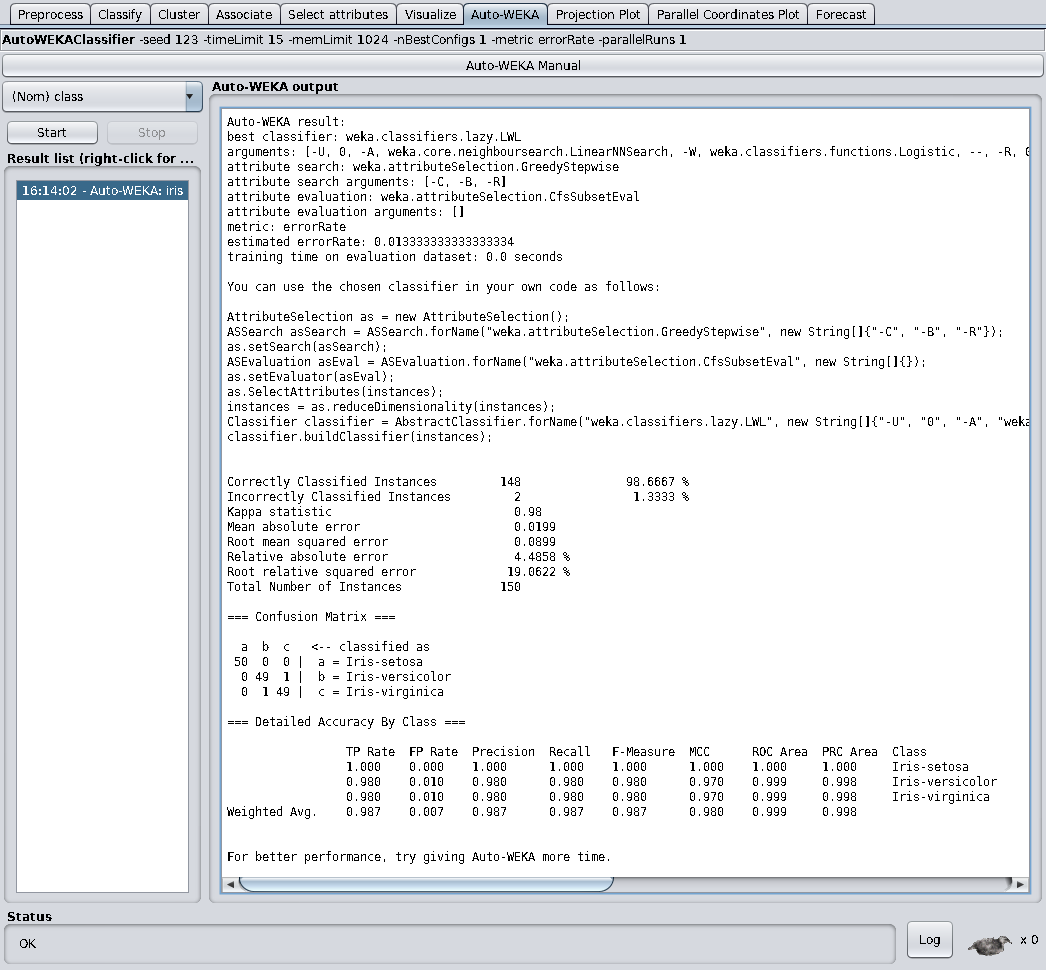
\includegraphics[width=.8\textwidth]{tab}
\caption{Auto-WEKA tab showing the output of a completed run.}
\label{fig:tab}
\end{center}
\end{figure}

Alternatively, Auto-WEKA can be run through the normal ``Classify'' panel by
selecting it from the list of classifiers (Figure~\ref{fig:classifier}).

\begin{figure}[!ht]
\begin{center}
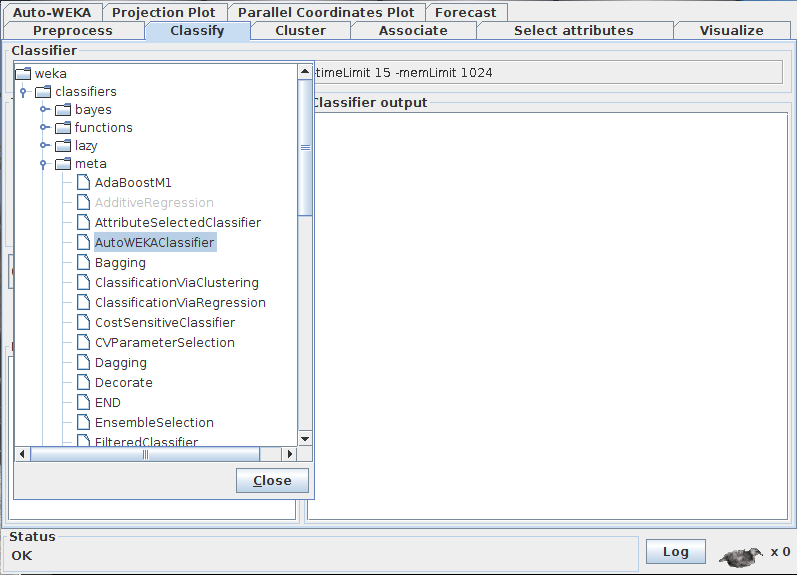
\includegraphics[width=.8\textwidth]{classifier}
\caption{Location of the Auto-WEKA classifier in the list of classifiers.}
\label{fig:classifier}
\end{center}
\end{figure}

When using Auto-WEKA like a normal classifier, it is important to select the
Test option ``Use training set''. Auto-WEKA performs a statistically rigorous
evaluation internally and does not require an external split into training and
test sets that WEKA provides. Not selecting this option will not improve the
quality of the result and cause Auto-WEKA to take much longer.
Figure~\ref{fig:train} shows the recommended setting.

\begin{figure}[!ht]
\begin{center}
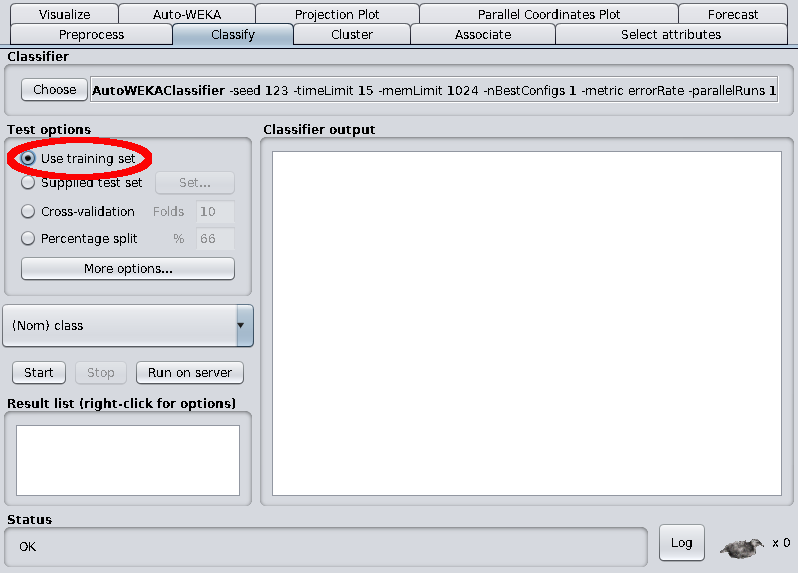
\includegraphics[width=.8\textwidth]{train}
\caption{Recommended evaluation setting when using Auto-WEKA like a normal
classifier.}
\label{fig:train}
\end{center}
\end{figure}

Auto-WEKA has only a few options. Figure~\ref{fig:options} shows them. Usually,
you can leave them at their default values. For most users, only two options are
relevant:
\begin{description}
\item[timeLimit] The time in minutes Auto-WEKA will take to determine the best
classifier and configuration. If you get bad results, try increasing this value.
\item[memLimit] The memory limit in Megabytes for running classifiers. If you
have a very large dataset, you may need to increase this value.
\end{description}

\begin{figure}[!ht]
\begin{center}
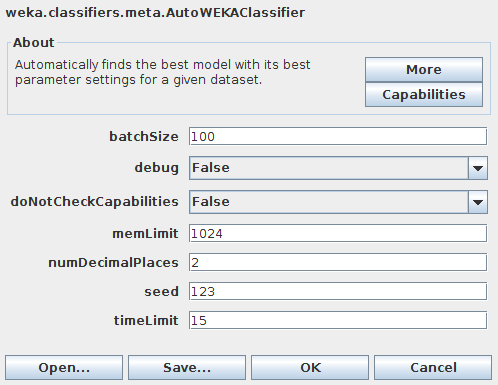
\includegraphics[width=.8\textwidth]{options}
\caption{Auto-WEKA options.}
\label{fig:options}
\end{center}
\end{figure}

While Auto-WEKA is running, it will provide the number of evaluated
configurations and estimated error of the best configuration found so far in the
status bar.

\medskip

Note that the time limit is \emph{approximate} and Auto-WEKA may not take
\emph{exactly} as long as requested.

%%%%%%%%%%%%%%%%%%%%%%%%%%%%%%%%%%%%%%%%%%% 
\subsection{Running Experiments Using the CLI}\label{sec:running}
%%%%%%%%%%%%%%%%%%%%%%%%%%%%%%%%%%%%%%%%%%%

Auto-WEKA can be run from the CLI like any other WEKA classifier, for example:
\begin{verbatim}
java -cp autoweka.jar weka.classifiers.meta.AutoWEKAClassifier \
    -t iris.arff -timeLimit 15 -no-cv
\end{verbatim}
 
\end{document}
